\section{Views}
\label{sec:ui_views}

The 'Add View' button \includegraphics[width=0.5cm,frame]{../../data/icons/crosshair_fat.png} on the top right in each window allows adding views to the current window or in a new window. \\

Each View is contained in a tab within a parent window.  At startup, per default only the main window exists, which also holds
a Geographic View and a Table view. If the main window is closed, the COMPASS client shuts down. New Views can be added using the 'Add View' button, which opens a pull-down menu. Each View can either be added to the main window ('Add Here') or into a new window ('Add in New Window'. When added, a new tab exists in the containing window. \\

New Views can be added either to currently existing windows as new tabs, or to a newly opened window. A window can be closed either by the close button in the window decoration, which discards all contained Views within the window.  \\

To close a single View, one can use the \includegraphics[width=0.5cm,frame]{../../data/icons/edit.png} button in the tab header and press 'Close'.
This also frees all of the View's allocated resources. \\

Each View adds its required variables to the loading list for the database. During a loading process, the loading status of a View is shown in its Configuration Panel.\\

Currently, the following Views exist:
\begin{itemize}
 \item \nameref{sec:histo_view}
 \item \nameref{sec:table_view}
 \item \nameref{sec:geo_view}
 \item \nameref{sec:scatter_view}
 \item \nameref{sec:grid_view}
\end{itemize}

\subsection{View Presets}

A view can typically be configured via the Configuration Panel on its right side.
A view preset represents the state of this configuration for a certain kind of view,
which can be saved and restored at a later point for a specific display use case. 
Such a use case could for instance be a certain kind of assessment carried out by the user
on a regular basis. By making use of view presets, users can restore often used view configurations conveniently. \\

Please \textbf{note} that view presets are created for a certain type of view (Geographic View, HistogramView, etc.),
and are always shared amongst these views. For each type of view, a number of pre-defined \textit{default presets} are deployed with a new COMPASS release. \\

In the toolbar of each view, the view preset selection is shown on the left side. 

\begin{figure}[H]
    \center
    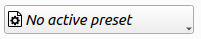
\includegraphics[width=4cm]{figures/view_preset_selection.png}
  \caption{View Preset Selection}
\end{figure}

It displays the name of the last applied preset, if no preset has been applied it shows \textit{No active preset}.
If the view configuration has been modified since a preset has been applied, a change indicator (*) is displayed after the preset name.

\begin{figure}[H]
    \center
    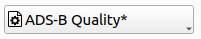
\includegraphics[width=4cm]{figures/view_preset_selection_modified.png}
  \caption{View Preset Selection - Modified Preset}
\end{figure}

When clicked, the view preset list opens:

\begin{figure}[H]
    \center
    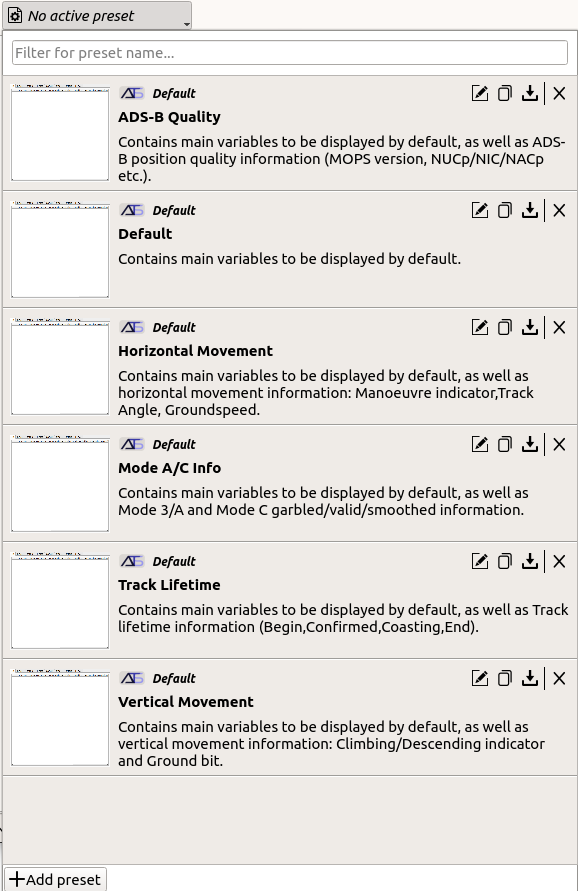
\includegraphics[width=10cm,frame]{figures/view_presets.png}
  \caption{View Preset Selection - Preset List}
\end{figure}

All view presets existing for the current type of view are listed, and can be applied with a single left click on a preset item. 
Applying the preset will reconfigure the view and refresh it accordingly. \\

Please \textbf{note} that if a view preset is selected, the configuration is applied immediately, often triggering a reload of the surveillance data. \\

A preset item contains the following information:

\begin{itemize}
 \item \textbf{Screenshot}: A screenshot of the view, taken when the preset is created/saved, serving as a preview image for the preset
 \item \textbf{Preset Origin}: Icon, showing where the preset originates from, either 
\includegraphics[width=0.5cm,frame]{figures/view_presets_origin_openats.png} (delivered with the application) 
 or 
\includegraphics[width=0.5cm,frame]{figures/view_presets_origin_user.png} (created by user)
 \item \textbf{Category}: Optional preset category
 \item \textbf{Name}: A (unique) descriptive name
 \item \textbf{Description}: An optional description of the preset
\end{itemize} \ \\

Additionally, a number of actions exist for each preset:

\begin{itemize}
 \item \includegraphics[width=0.5cm,frame]{../../data/icons/edit_old.png}: \textit{Edit} the preset's meta-information (category, description)
 \item 
\includegraphics[width=0.5cm,frame]{../../data/icons/copy.png}: \textit{Copy} the preset into a new one
 \item \includegraphics[width=0.5cm,frame]{../../data/icons/save.png}: \textit{Save} the current view configuration into the preset
 \item \includegraphics[width=0.5cm,frame]{../../data/icons/delete.png}: \textit{Delete} the preset
\end{itemize} \ \\

Please \textbf{note} that since presets are shared amongst a certain type of view (e.g. Geographic View), applying these actions to a preset 
will alter the preset for all views of the same type. \\

\textit{Example}: Deleting a preset in Geographic View will remove the preset for all currently existing and future Geographic Views. \\

Each type of action will be described in more detail below:

\paragraph*{Edit} The category and description of a preset can be edited by clicking the \textit{edit} action, which opens the following dialog:

\begin{figure}[H]
    \center
    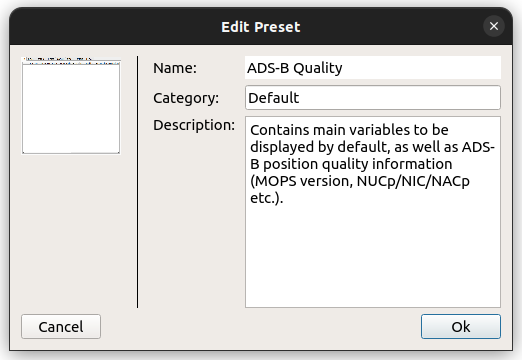
\includegraphics[width=10cm]{figures/view_preset_edit.png}
  \caption{View Preset Editing}
\end{figure}

\paragraph*{Copy} A preset can be copied to a new preset by clicking the \textit{copy} action, which opens the following dialog:

\begin{figure}[H]
    \center
    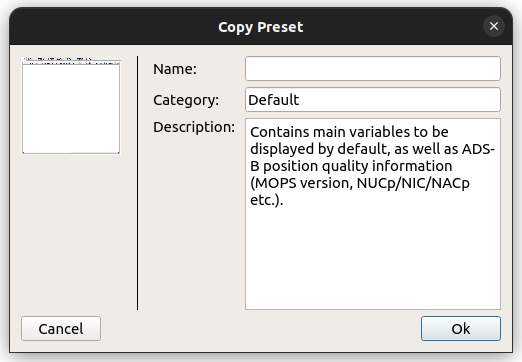
\includegraphics[width=10cm]{figures/view_preset_copy.png}
  \caption{View Preset Copying}
\end{figure}

Then a new (unique) name can be specified for the copied preset, and the category and description can be edited.
The view configuration stored in the copied preset will be transferred to the new preset.

\paragraph*{Save} The current view configuration can be saved to an existing preset by clicking the \textit{Save} action \includegraphics[width=0.5cm,frame]{../../data/icons/save.png}. \\

Please \textbf{note} that if changes are made in the configuration tab of a view, these changes are not saved to a preset automatically. 
Such an action has to be performed manually by the user using this functionality.

\paragraph*{Delete} A preset can be deleted by clicking the \textit{delete} action.
In the case of a default preset (a preset delivered with the application), the user will be prompted if the preset should really
be deleted. \\

Please \textbf{note} that presets will be deleted \textbf{permanently}, so once removed, default presets cannot be recovered easily.

\paragraph*{Creating New Presets} The \textit{Add preset} button resides at the bottom of the preset list, 
and can be used to create a new preset from the current view configuration. Clicking the button will open the following dialog:

\begin{figure}[H]
    \center
    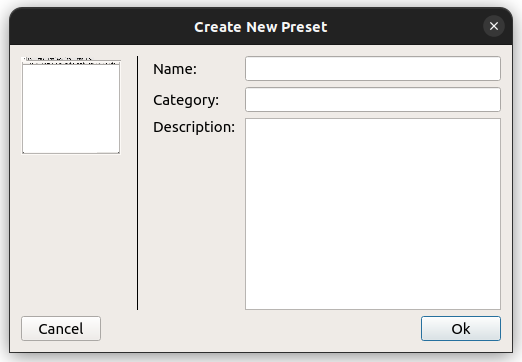
\includegraphics[width=10cm]{figures/view_preset_add.png}
  \caption{Creating a New Preset} 
\end{figure}

A unique name has to be be specified. Optionally, a category and description for the new preset can be entered.

\paragraph*{Filtering Presets} At the top of the preset list, a filter text field resides, which can be used to filter presets by name.

\begin{figure}[H]
    \center
    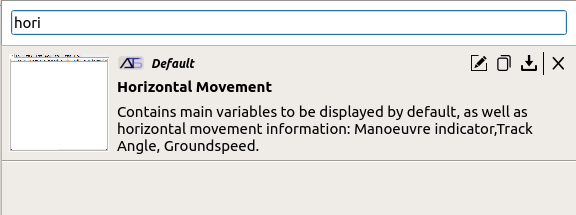
\includegraphics[width=10cm]{figures/view_preset_filter.png}
  \caption{Filtering Presets by Name}
\end{figure}

\paragraph*{Presets and COMPASS Version}

Please \textbf{note} that user-created view presets are always created for the currently running COMPASS version, 
and have to be recreated manually each time a COMPASS version upgrade is performed. \\

If this is cumbersome, or if a specific view preset should added to the list of default presets officially deployed with compass, 
please contact \href{mailto:compass@openats.at}{compass@openats.at} for support.

\subsection{View Cross Selection}

A very convenient feature which is supported by all views is cross selection of data. Data items selected in one view will also be highlighted in all other views, 
allowing for closer inspection of data portions across multiple views. This selection also persists if a reload is triggered either in the main window or in a view. \\

Selected data items will be highlighted in a special way, typically in yellow color. In Table View a checkbox will be set for selected data items.

\paragraph*{Example} In the image below a certain slice of time is selected in Histogram View. 
The target reports belonging to this time frame will also be selected in Geographic View.

\begin{figure}[H]
  \hspace*{-2.5cm}
  \center
  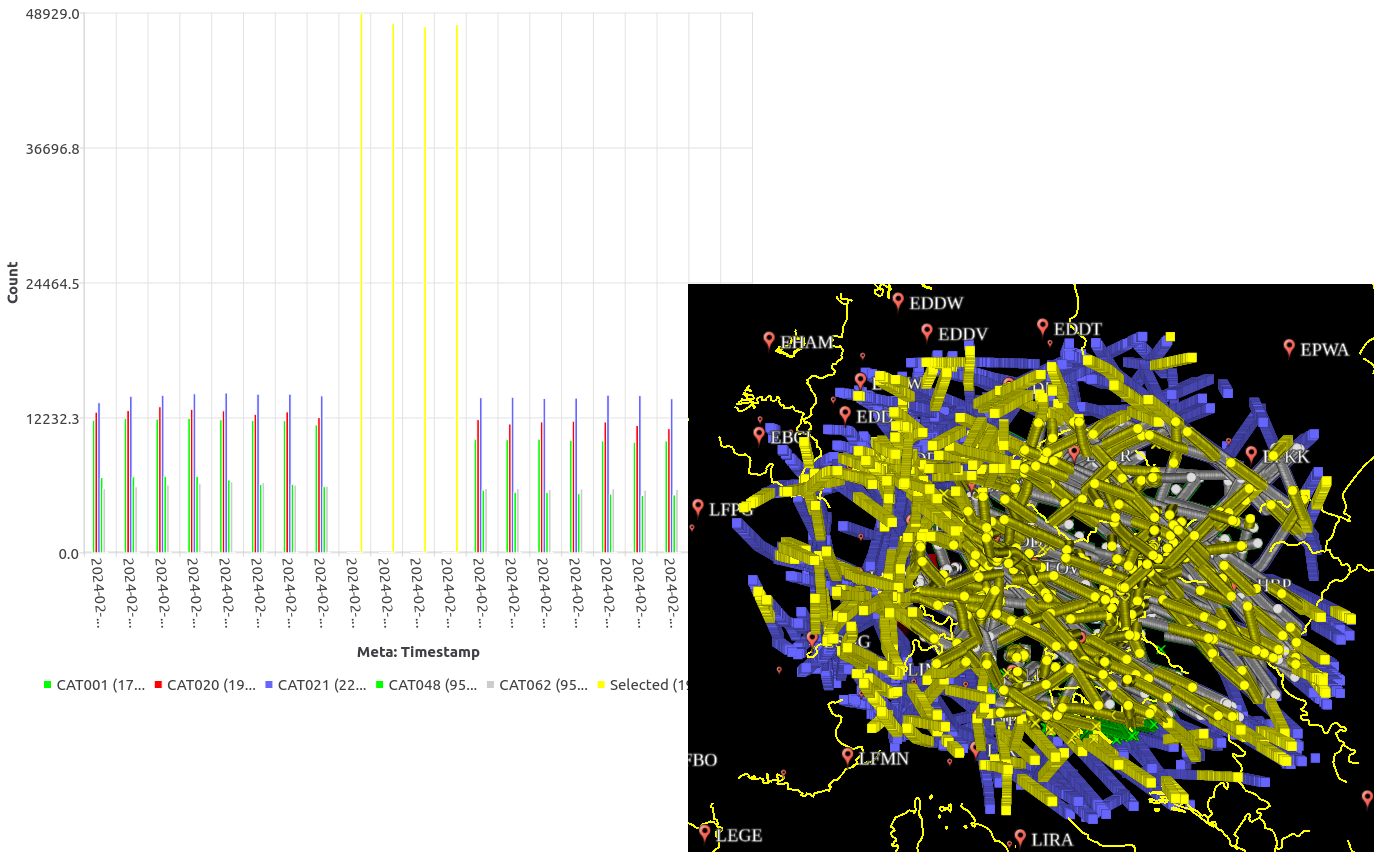
\includegraphics[width=19cm]{figures/cross_selection.png}
  \caption{Cross Selection}
\end{figure}

\subsection{Plots and Plot Groups}
\label{sec:plots}

Some Views support the concept of showing a \textit{Plot}, which represents a single displayable item in this view, 
such as a histogram, a scatter point series, gridded data, etc. If such displayable Plot annotation data is present (e.g. provided by a Viewpoint, see \nameref{sec:view_points}), 
it can be selected in the Configuration Panel of the View by switching to 'Show Annotations' and using the 'Plot' combo box.

\begin{figure}[H]
  \hspace*{-0.5cm}
  \center
  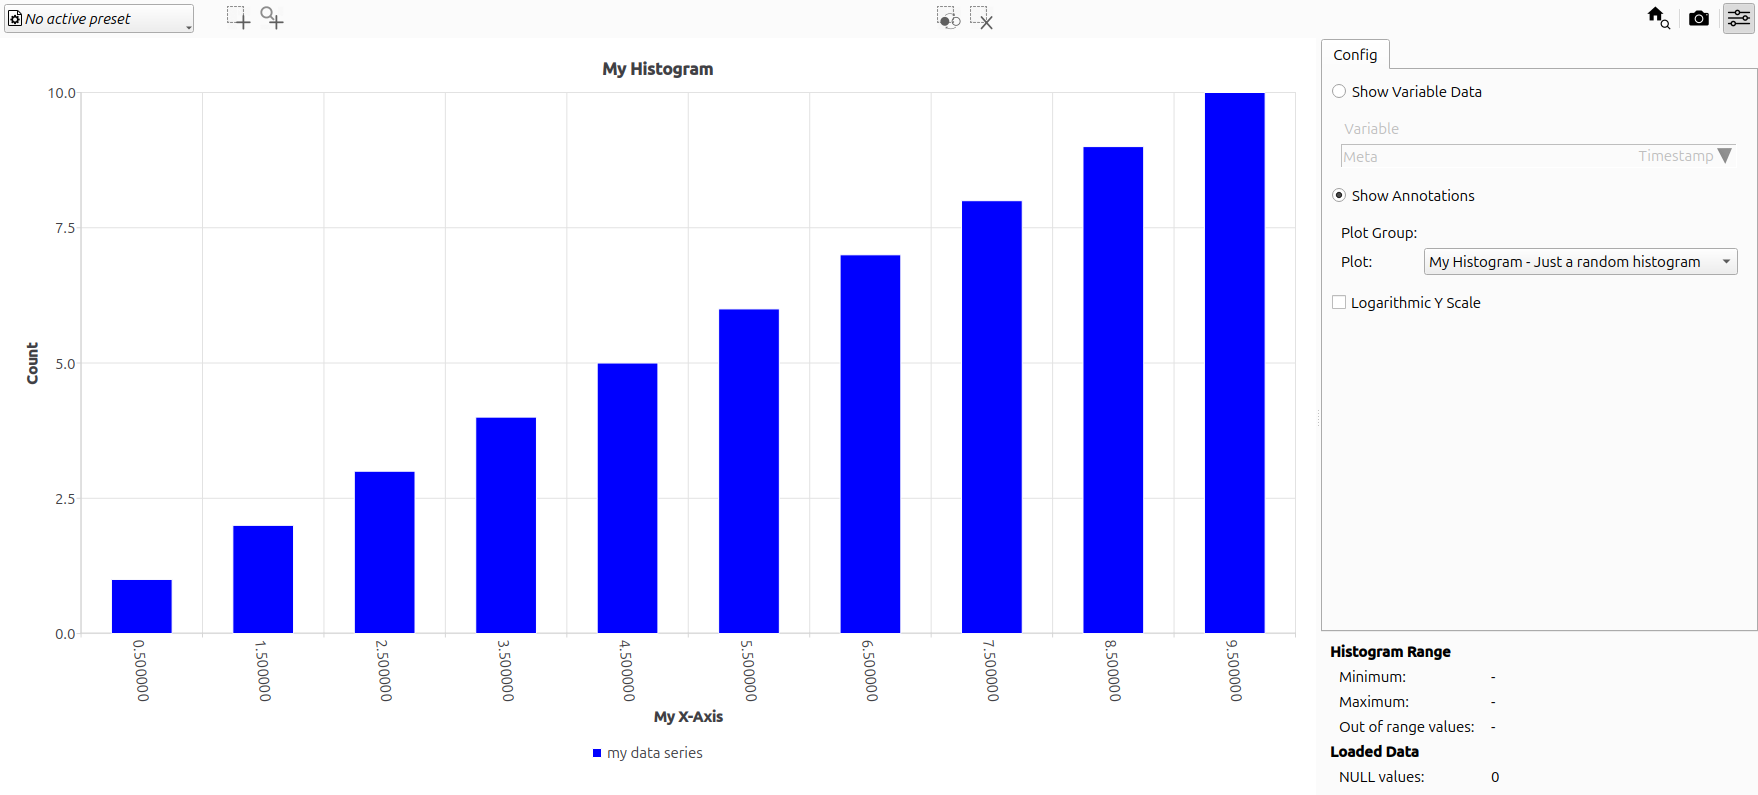
\includegraphics[width=18cm]{figures/view_select_plot.png}
\caption{Histogram View: Selecting a Plot item}
\end{figure}

Plots might further be grouped into so-called \textit{Plot Groups}. A Plot Group can be selected by using the 'Plot Group' combo box, if available.

\begin{figure}[H]
  \hspace*{-0.5cm}
  \center
  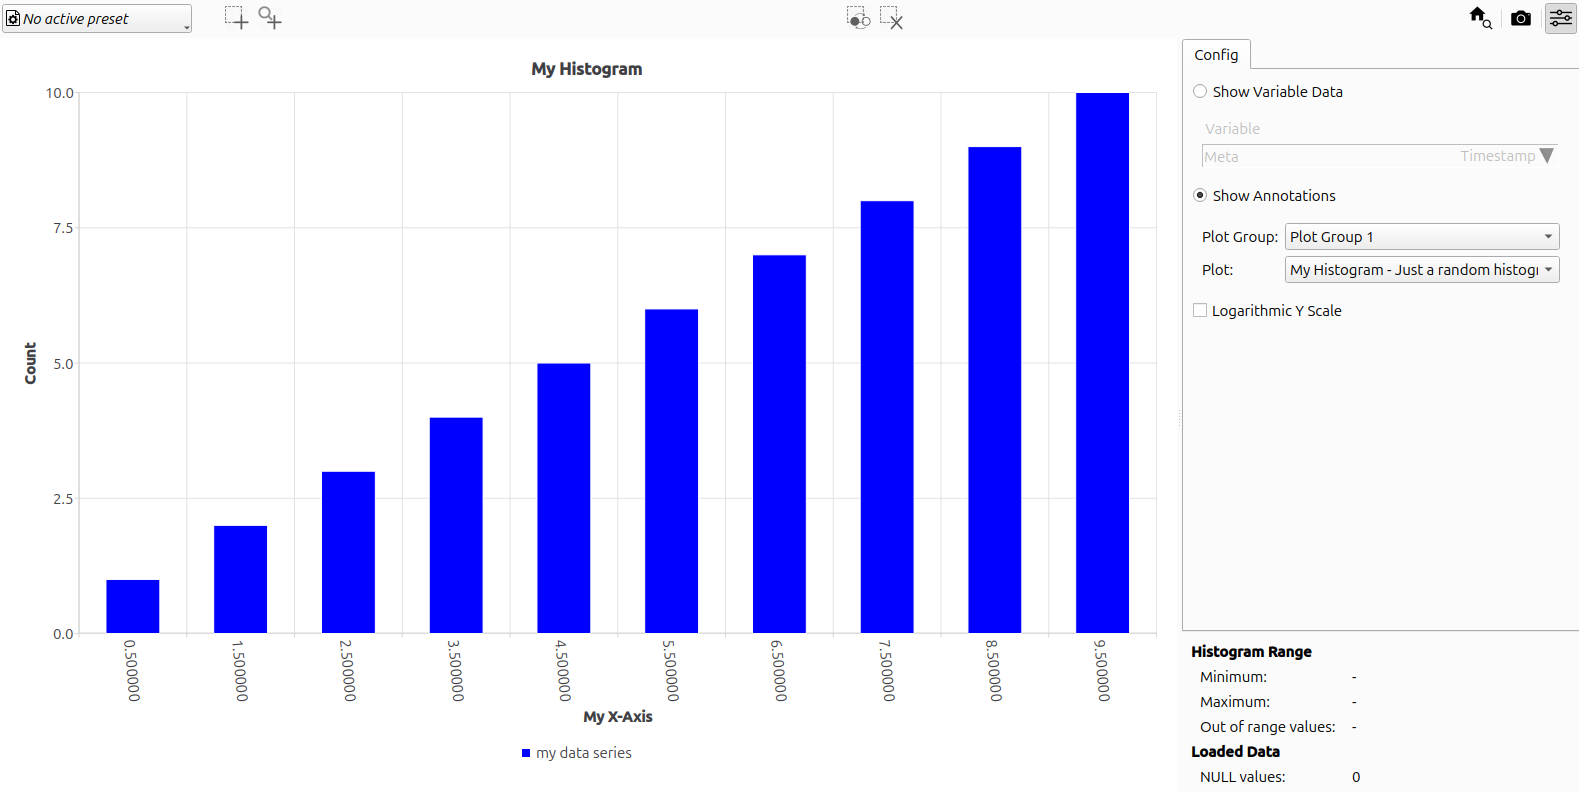
\includegraphics[width=18cm]{figures/view_select_plot_group.png}
\caption{Histogram View: Selecting a Plot Group}
\end{figure}

At the moment the following Views support the concept of Plots:

\begin{itemize}
  \item Histogram View
  \item Scatterplot View
  \item Grid View
 \end{itemize} \ \\
 